\documentclass[11pt,compress,t,notes=noshow, xcolor=table]{beamer}

\usepackage[]{graphicx}\usepackage[]{color}
% maxwidth is the original width if it is less than linewidth
% otherwise use linewidth (to make sure the graphics do not exceed the margin)
\makeatletter
\def\maxwidth{ %
  \ifdim\Gin@nat@width>\linewidth
    \linewidth
  \else
    \Gin@nat@width
  \fi
}
\makeatother

\definecolor{fgcolor}{rgb}{0.345, 0.345, 0.345}
\newcommand{\hlnum}[1]{\textcolor[rgb]{0.686,0.059,0.569}{#1}}%
\newcommand{\hlstr}[1]{\textcolor[rgb]{0.192,0.494,0.8}{#1}}%
\newcommand{\hlcom}[1]{\textcolor[rgb]{0.678,0.584,0.686}{\textit{#1}}}%
\newcommand{\hlopt}[1]{\textcolor[rgb]{0,0,0}{#1}}%
\newcommand{\hlstd}[1]{\textcolor[rgb]{0.345,0.345,0.345}{#1}}%
\newcommand{\hlkwa}[1]{\textcolor[rgb]{0.161,0.373,0.58}{\textbf{#1}}}%
\newcommand{\hlkwb}[1]{\textcolor[rgb]{0.69,0.353,0.396}{#1}}%
\newcommand{\hlkwc}[1]{\textcolor[rgb]{0.333,0.667,0.333}{#1}}%
\newcommand{\hlkwd}[1]{\textcolor[rgb]{0.737,0.353,0.396}{\textbf{#1}}}%
\let\hlipl\hlkwb

\usepackage{framed}
\makeatletter
\newenvironment{kframe}{%
 \def\at@end@of@kframe{}%
 \ifinner\ifhmode%
  \def\at@end@of@kframe{\end{minipage}}%
  \begin{minipage}{\columnwidth}%
 \fi\fi%
 \def\FrameCommand##1{\hskip\@totalleftmargin \hskip-\fboxsep
 \colorbox{shadecolor}{##1}\hskip-\fboxsep
     % There is no \\@totalrightmargin, so:
     \hskip-\linewidth \hskip-\@totalleftmargin \hskip\columnwidth}%
 \MakeFramed {\advance\hsize-\width
   \@totalleftmargin\z@ \linewidth\hsize
   \@setminipage}}%
 {\par\unskip\endMakeFramed%
 \at@end@of@kframe}
\makeatother

\definecolor{shadecolor}{rgb}{.97, .97, .97}
\definecolor{messagecolor}{rgb}{0, 0, 0}
\definecolor{warningcolor}{rgb}{1, 0, 1}
\definecolor{errorcolor}{rgb}{1, 0, 0}
\newenvironment{knitrout}{}{} % an empty environment to be redefined in TeX

\usepackage{alltt}
\newcommand{\SweaveOpts}[1]{}  % do not interfere with LaTeX
\newcommand{\SweaveInput}[1]{} % because they are not real TeX commands
\newcommand{\Sexpr}[1]{}       % will only be parsed by R
\newcommand{\xmark}{\ding{55}}%


\usepackage[english]{babel}
\usepackage[utf8]{inputenc}

\usepackage{dsfont}
\usepackage{verbatim}
\usepackage{amsmath}
\usepackage{amsfonts}
\usepackage{amssymb}
\usepackage{bm}
\usepackage{csquotes}
\usepackage{multirow}
\usepackage{longtable}
\usepackage{booktabs}
\usepackage{enumerate}
\usepackage[absolute,overlay]{textpos}
\usepackage{psfrag}
\usepackage{algorithm}
\usepackage{algpseudocode}
\usepackage{eqnarray}
\usepackage{arydshln}
\usepackage{tabularx}
\usepackage{placeins}
\usepackage{tikz}
\usepackage{setspace}
\usepackage{colortbl}
\usepackage{mathtools}
\usepackage{wrapfig}
\usepackage{bm}
\usepackage{amsmath}
\usepackage{pifont}

\usetikzlibrary{shapes,arrows,automata,positioning,calc,chains,trees, shadows}
\tikzset{
  %Define standard arrow tip
  >=stealth',
  %Define style for boxes
  punkt/.style={
    rectangle,
    rounded corners,
    draw=black, very thick,
    text width=6.5em,
    minimum height=2em,
    text centered},
  % Define arrow style
  pil/.style={
    ->,
    thick,
    shorten <=2pt,
    shorten >=2pt,}
}

\usepackage{subfig}

% Defines macros and environments
\usepackage{../../style/lmu-lecture}


\let\code=\texttt
\let\proglang=\textsf

\setkeys{Gin}{width=0.9\textwidth}

\setbeamertemplate{frametitle}{\expandafter\uppercase\expandafter\insertframetitle}

\usepackage{bbm}
% basic latex stuff
\newcommand{\pkg}[1]{{\fontseries{b}\selectfont #1}} %fontstyle for R packages
\newcommand{\lz}{\vspace{0.5cm}} %vertical space
\newcommand{\dlz}{\vspace{1cm}} %double vertical space
\newcommand{\oneliner}[1] % Oneliner for important statements
{\begin{block}{}\begin{center}\begin{Large}#1\end{Large}\end{center}\end{block}}


%new environments
\newenvironment{vbframe}  %frame with breaks and verbatim
{
 \begin{frame}[containsverbatim,allowframebreaks]
}
{
\end{frame}
}

\newenvironment{vframe}  %frame with verbatim without breaks (to avoid numbering one slided frames)
{
 \begin{frame}[containsverbatim]
}
{
\end{frame}
}

\newenvironment{blocki}[1]   % itemize block
{
 \begin{block}{#1}\begin{itemize}
}
{
\end{itemize}\end{block}
}

\newenvironment{fragileframe}[2]{  %fragile frame with framebreaks
\begin{frame}[allowframebreaks, fragile, environment = fragileframe]
\frametitle{#1}
#2}
{\end{frame}}


\newcommand{\myframe}[2]{  %short for frame with framebreaks
\begin{frame}[allowframebreaks]
\frametitle{#1}
#2
\end{frame}}

\newcommand{\remark}[1]{
  \textbf{Remark:} #1
}


\newenvironment{deleteframe}
{
\begingroup
\usebackgroundtemplate{
\includegraphics[width=\paperwidth,height=\paperheight]{../style/color/red.png}}
 \begin{frame}
}
{
\end{frame}
\endgroup
}
\newenvironment{simplifyframe}
{
\begingroup
\usebackgroundtemplate{
\includegraphics[width=\paperwidth,height=\paperheight]{../style/color/yellow.png}}
 \begin{frame}
}
{
\end{frame}
\endgroup
}\newenvironment{draftframe}
{
\begingroup
\usebackgroundtemplate{
\includegraphics[width=\paperwidth,height=\paperheight]{../style/color/green.jpg}}
 \begin{frame}
}
{
\end{frame}
\endgroup
}
% https://tex.stackexchange.com/a/261480: textcolor that works in mathmode
\makeatletter
\renewcommand*{\@textcolor}[3]{%
  \protect\leavevmode
  \begingroup
    \color#1{#2}#3%
  \endgroup
}
\makeatother





% math spaces
\ifdefined\N                                                                
\renewcommand{\N}{\mathds{N}} % N, naturals
\else \newcommand{\N}{\mathds{N}} \fi 
\newcommand{\Z}{\mathds{Z}} % Z, integers
\newcommand{\Q}{\mathds{Q}} % Q, rationals
\newcommand{\R}{\mathds{R}} % R, reals
\ifdefined\C 
  \renewcommand{\C}{\mathds{C}} % C, complex
\else \newcommand{\C}{\mathds{C}} \fi
\newcommand{\continuous}{\mathcal{C}} % C, space of continuous functions
\newcommand{\M}{\mathcal{M}} % machine numbers
\newcommand{\epsm}{\epsilon_m} % maximum error

% counting / finite sets
\newcommand{\setzo}{\{0, 1\}} % set 0, 1
\newcommand{\setmp}{\{-1, +1\}} % set -1, 1
\newcommand{\unitint}{[0, 1]} % unit interval

% basic math stuff
\newcommand{\xt}{\tilde x} % x tilde
\newcommand{\argmax}{\operatorname{arg\,max}} % argmax
\newcommand{\argmin}{\operatorname{arg\,min}} % argmin
\newcommand{\argminlim}{\mathop{\mathrm{arg\,min}}\limits} % argmax with limits
\newcommand{\argmaxlim}{\mathop{\mathrm{arg\,max}}\limits} % argmin with limits  
\newcommand{\sign}{\operatorname{sign}} % sign, signum
\newcommand{\I}{\mathbb{I}} % I, indicator
\newcommand{\order}{\mathcal{O}} % O, order
\newcommand{\pd}[2]{\frac{\partial{#1}}{\partial #2}} % partial derivative
\newcommand{\floorlr}[1]{\left\lfloor #1 \right\rfloor} % floor
\newcommand{\ceillr}[1]{\left\lceil #1 \right\rceil} % ceiling

% sums and products
\newcommand{\sumin}{\sum\limits_{i=1}^n} % summation from i=1 to n
\newcommand{\sumim}{\sum\limits_{i=1}^m} % summation from i=1 to m
\newcommand{\sumjn}{\sum\limits_{j=1}^n} % summation from j=1 to p
\newcommand{\sumjp}{\sum\limits_{j=1}^p} % summation from j=1 to p
\newcommand{\sumik}{\sum\limits_{i=1}^k} % summation from i=1 to k
\newcommand{\sumkg}{\sum\limits_{k=1}^g} % summation from k=1 to g
\newcommand{\sumjg}{\sum\limits_{j=1}^g} % summation from j=1 to g
\newcommand{\meanin}{\frac{1}{n} \sum\limits_{i=1}^n} % mean from i=1 to n
\newcommand{\meanim}{\frac{1}{m} \sum\limits_{i=1}^m} % mean from i=1 to n
\newcommand{\meankg}{\frac{1}{g} \sum\limits_{k=1}^g} % mean from k=1 to g
\newcommand{\prodin}{\prod\limits_{i=1}^n} % product from i=1 to n
\newcommand{\prodkg}{\prod\limits_{k=1}^g} % product from k=1 to g
\newcommand{\prodjp}{\prod\limits_{j=1}^p} % product from j=1 to p

% linear algebra
\newcommand{\one}{\boldsymbol{1}} % 1, unitvector
\newcommand{\zero}{\mathbf{0}} % 0-vector
\newcommand{\id}{\boldsymbol{I}} % I, identity
\newcommand{\diag}{\operatorname{diag}} % diag, diagonal
\newcommand{\trace}{\operatorname{tr}} % tr, trace
\newcommand{\spn}{\operatorname{span}} % span
\newcommand{\scp}[2]{\left\langle #1, #2 \right\rangle} % <.,.>, scalarproduct
\newcommand{\mat}[1]{\begin{pmatrix} #1 \end{pmatrix}} % short pmatrix command
\newcommand{\Amat}{\mathbf{A}} % matrix A
\newcommand{\Deltab}{\mathbf{\Delta}} % error term for vectors

% basic probability + stats
\renewcommand{\P}{\mathds{P}} % P, probability
\newcommand{\E}{\mathds{E}} % E, expectation
\newcommand{\var}{\mathsf{Var}} % Var, variance
\newcommand{\cov}{\mathsf{Cov}} % Cov, covariance
\newcommand{\corr}{\mathsf{Corr}} % Corr, correlation
\newcommand{\normal}{\mathcal{N}} % N of the normal distribution
\newcommand{\iid}{\overset{i.i.d}{\sim}} % dist with i.i.d superscript
\newcommand{\distas}[1]{\overset{#1}{\sim}} % ... is distributed as ...

% machine learning
\newcommand{\Xspace}{\mathcal{X}} % X, input space
\newcommand{\Yspace}{\mathcal{Y}} % Y, output space
\newcommand{\nset}{\{1, \ldots, n\}} % set from 1 to n
\newcommand{\pset}{\{1, \ldots, p\}} % set from 1 to p
\newcommand{\gset}{\{1, \ldots, g\}} % set from 1 to g
\newcommand{\Pxy}{\mathbb{P}_{xy}} % P_xy
\newcommand{\Exy}{\mathbb{E}_{xy}} % E_xy: Expectation over random variables xy
\newcommand{\xv}{\mathbf{x}} % vector x (bold)
\newcommand{\xtil}{\tilde{\mathbf{x}}} % vector x-tilde (bold)
\newcommand{\yv}{\mathbf{y}} % vector y (bold)
\newcommand{\xy}{(\xv, y)} % observation (x, y)
\newcommand{\xvec}{\left(x_1, \ldots, x_p\right)^\top} % (x1, ..., xp) 
\newcommand{\Xmat}{\mathbf{X}} % Design matrix
\newcommand{\allDatasets}{\mathds{D}} % The set of all datasets
\newcommand{\allDatasetsn}{\mathds{D}_n}  % The set of all datasets of size n 
\newcommand{\D}{\mathcal{D}} % D, data
\newcommand{\Dn}{\D_n} % D_n, data of size n
\newcommand{\Dtrain}{\mathcal{D}_{\text{train}}} % D_train, training set
\newcommand{\Dtest}{\mathcal{D}_{\text{test}}} % D_test, test set
\newcommand{\xyi}[1][i]{\left(\xv^{(#1)}, y^{(#1)}\right)} % (x^i, y^i), i-th observation
\newcommand{\Dset}{\left( \xyi[1], \ldots, \xyi[n]\right)} % {(x1,y1)), ..., (xn,yn)}, data
\newcommand{\defAllDatasetsn}{(\Xspace \times \Yspace)^n} % Def. of the set of all datasets of size n 
\newcommand{\defAllDatasets}{\bigcup_{n \in \N}(\Xspace \times \Yspace)^n} % Def. of the set of all datasets 
\newcommand{\xdat}{\left\{ \xv^{(1)}, \ldots, \xv^{(n)}\right\}} % {x1, ..., xn}, input data
\newcommand{\yvec}{\left(y^{(1)}, \hdots, y^{(n)}\right)^\top} % (y1, ..., yn), vector of outcomes
\renewcommand{\xi}[1][i]{\xv^{(#1)}} % x^i, i-th observed value of x
\newcommand{\yi}[1][i]{y^{(#1)}} % y^i, i-th observed value of y 
\newcommand{\xivec}{\left(x^{(i)}_1, \ldots, x^{(i)}_p\right)^\top} % (x1^i, ..., xp^i), i-th observation vector
\newcommand{\xj}{\xv_j} % x_j, j-th feature
\newcommand{\xjvec}{\left(x^{(1)}_j, \ldots, x^{(n)}_j\right)^\top} % (x^1_j, ..., x^n_j), j-th feature vector
\newcommand{\phiv}{\mathbf{\phi}} % Basis transformation function phi
\newcommand{\phixi}{\mathbf{\phi}^{(i)}} % Basis transformation of xi: phi^i := phi(xi)

%%%%%% ml - models general
\newcommand{\lamv}{\bm{\lambda}} % lambda vector, hyperconfiguration vector
\newcommand{\Lam}{\bm{\Lambda}}	 % Lambda, space of all hpos
% Inducer / Inducing algorithm
\newcommand{\preimageInducer}{\left(\defAllDatasets\right)\times\Lam} % Set of all datasets times the hyperparameter space
\newcommand{\preimageInducerShort}{\allDatasets\times\Lam} % Set of all datasets times the hyperparameter space
% Inducer / Inducing algorithm
\newcommand{\ind}{\mathcal{I}} % Inducer, inducing algorithm, learning algorithm 

% continuous prediction function f
\newcommand{\ftrue}{f_{\text{true}}}  % True underlying function (if a statistical model is assumed)
\newcommand{\ftruex}{\ftrue(\xv)} % True underlying function (if a statistical model is assumed)
\newcommand{\fx}{f(\xv)} % f(x), continuous prediction function
\newcommand{\fdomains}{f: \Xspace \rightarrow \R^g} % f with domain and co-domain
\newcommand{\Hspace}{\mathcal{H}} % hypothesis space where f is from
\newcommand{\fbayes}{f^{\ast}} % Bayes-optimal model
\newcommand{\fxbayes}{f^{\ast}(\xv)} % Bayes-optimal model
\newcommand{\fkx}[1][k]{f_{#1}(\xv)} % f_j(x), discriminant component function
\newcommand{\fh}{\hat{f}} % f hat, estimated prediction function
\newcommand{\fxh}{\fh(\xv)} % fhat(x)
\newcommand{\fxt}{f(\xv ~|~ \thetab)} % f(x | theta)
\newcommand{\fxi}{f\left(\xv^{(i)}\right)} % f(x^(i))
\newcommand{\fxih}{\hat{f}\left(\xv^{(i)}\right)} % f(x^(i))
\newcommand{\fxit}{f\left(\xv^{(i)} ~|~ \thetab\right)} % f(x^(i) | theta)
\newcommand{\fhD}{\fh_{\D}} % fhat_D, estimate of f based on D
\newcommand{\fhDtrain}{\fh_{\Dtrain}} % fhat_Dtrain, estimate of f based on D
\newcommand{\fhDnlam}{\fh_{\Dn, \lamv}} %model learned on Dn with hp lambda
\newcommand{\fhDlam}{\fh_{\D, \lamv}} %model learned on D with hp lambda
\newcommand{\fhDnlams}{\fh_{\Dn, \lamv^\ast}} %model learned on Dn with optimal hp lambda 
\newcommand{\fhDlams}{\fh_{\D, \lamv^\ast}} %model learned on D with optimal hp lambda 

% discrete prediction function h
\newcommand{\hx}{h(\xv)} % h(x), discrete prediction function
\newcommand{\hh}{\hat{h}} % h hat
\newcommand{\hxh}{\hat{h}(\xv)} % hhat(x)
\newcommand{\hxt}{h(\xv | \thetab)} % h(x | theta)
\newcommand{\hxi}{h\left(\xi\right)} % h(x^(i))
\newcommand{\hxit}{h\left(\xi ~|~ \thetab\right)} % h(x^(i) | theta)
\newcommand{\hbayes}{h^{\ast}} % Bayes-optimal classification model
\newcommand{\hxbayes}{h^{\ast}(\xv)} % Bayes-optimal classification model

% yhat
\newcommand{\yh}{\hat{y}} % yhat for prediction of target
\newcommand{\yih}{\hat{y}^{(i)}} % yhat^(i) for prediction of ith targiet
\newcommand{\resi}{\yi- \yih}

% theta
\newcommand{\thetah}{\hat{\theta}} % theta hat
\newcommand{\thetab}{\bm{\theta}} % theta vector
\newcommand{\thetabh}{\bm{\hat\theta}} % theta vector hat
\newcommand{\thetat}[1][t]{\thetab^{[#1]}} % theta^[t] in optimization
\newcommand{\thetatn}[1][t]{\thetab^{[#1 +1]}} % theta^[t+1] in optimization
\newcommand{\thetahDnlam}{\thetabh_{\Dn, \lamv}} %theta learned on Dn with hp lambda
\newcommand{\thetahDlam}{\thetabh_{\D, \lamv}} %theta learned on D with hp lambda
\newcommand{\mint}{\min_{\thetab \in \Theta}} % min problem theta
\newcommand{\argmint}{\argmin_{\thetab \in \Theta}} % argmin theta

% densities + probabilities
% pdf of x 
\newcommand{\pdf}{p} % p
\newcommand{\pdfx}{p(\xv)} % p(x)
\newcommand{\pixt}{\pi(\xv~|~ \thetab)} % pi(x|theta), pdf of x given theta
\newcommand{\pixit}{\pi\left(\xi ~|~ \thetab\right)} % pi(x^i|theta), pdf of x given theta
\newcommand{\pixii}{\pi\left(\xi\right)} % pi(x^i), pdf of i-th x 

% pdf of (x, y)
\newcommand{\pdfxy}{p(\xv,y)} % p(x, y)
\newcommand{\pdfxyt}{p(\xv, y ~|~ \thetab)} % p(x, y | theta)
\newcommand{\pdfxyit}{p\left(\xi, \yi ~|~ \thetab\right)} % p(x^(i), y^(i) | theta)

% pdf of x given y
\newcommand{\pdfxyk}[1][k]{p(\xv | y= #1)} % p(x | y = k)
\newcommand{\lpdfxyk}[1][k]{\log p(\xv | y= #1)} % log p(x | y = k)
\newcommand{\pdfxiyk}[1][k]{p\left(\xi | y= #1 \right)} % p(x^i | y = k)

% prior probabilities
\newcommand{\pik}[1][k]{\pi_{#1}} % pi_k, prior
\newcommand{\lpik}[1][k]{\log \pi_{#1}} % log pi_k, log of the prior
\newcommand{\pit}{\pi(\thetab)} % Prior probability of parameter theta

% posterior probabilities
\newcommand{\post}{\P(y = 1 ~|~ \xv)} % P(y = 1 | x), post. prob for y=1
\newcommand{\postk}[1][k]{\P(y = #1 ~|~ \xv)} % P(y = k | y), post. prob for y=k
\newcommand{\pidomains}{\pi: \Xspace \rightarrow \unitint} % pi with domain and co-domain
\newcommand{\pibayes}{\pi^{\ast}} % Bayes-optimal classification model
\newcommand{\pixbayes}{\pi^{\ast}(\xv)} % Bayes-optimal classification model
\newcommand{\pix}{\pi(\xv)} % pi(x), P(y = 1 | x)
\newcommand{\pikx}[1][k]{\pi_{#1}(\xv)} % pi_k(x), P(y = k | x)
\newcommand{\pikxt}[1][k]{\pi_{#1}(\xv ~|~ \thetab)} % pi_k(x | theta), P(y = k | x, theta)
\newcommand{\pixh}{\hat \pi(\xv)} % pi(x) hat, P(y = 1 | x) hat
\newcommand{\pikxh}[1][k]{\hat \pi_{#1}(\xv)} % pi_k(x) hat, P(y = k | x) hat
\newcommand{\pixih}{\hat \pi(\xi)} % pi(x^(i)) with hat
\newcommand{\pikxih}[1][k]{\hat \pi_{#1}(\xi)} % pi_k(x^(i)) with hat
\newcommand{\pdfygxt}{p(y ~|~\xv, \thetab)} % p(y | x, theta)
\newcommand{\pdfyigxit}{p\left(\yi ~|~\xi, \thetab\right)} % p(y^i |x^i, theta)
\newcommand{\lpdfygxt}{\log \pdfygxt } % log p(y | x, theta)
\newcommand{\lpdfyigxit}{\log \pdfyigxit} % log p(y^i |x^i, theta)

% probababilistic
\newcommand{\bayesrulek}[1][k]{\frac{\P(\xv | y= #1) \P(y= #1)}{\P(\xv)}} % Bayes rule
\newcommand{\muk}{\bm{\mu_k}} % mean vector of class-k Gaussian (discr analysis) 

% residual and margin
\newcommand{\eps}{\epsilon} % residual, stochastic
\newcommand{\epsi}{\epsilon^{(i)}} % epsilon^i, residual, stochastic
\newcommand{\epsh}{\hat{\epsilon}} % residual, estimated
\newcommand{\yf}{y \fx} % y f(x), margin
\newcommand{\yfi}{\yi \fxi} % y^i f(x^i), margin
\newcommand{\Sigmah}{\hat \Sigma} % estimated covariance matrix
\newcommand{\Sigmahj}{\hat \Sigma_j} % estimated covariance matrix for the j-th class

% ml - loss, risk, likelihood
\newcommand{\Lyf}{L\left(y, f\right)} % L(y, f), loss function
\newcommand{\Lxy}{L\left(y, \fx\right)} % L(y, f(x)), loss function
\newcommand{\Lxyi}{L\left(\yi, \fxi\right)} % loss of observation
\newcommand{\Lxyt}{L\left(y, \fxt\right)} % loss with f parameterized
\newcommand{\Lxyit}{L\left(\yi, \fxit\right)} % loss of observation with f parameterized
\newcommand{\Lxym}{L\left(\yi, f\left(\bm{\tilde{x}}^{(i)} ~|~ \thetab\right)\right)} % loss of observation with f parameterized
\newcommand{\Lpixy}{L\left(y, \pix\right)} % loss in classification
\newcommand{\Lpixyi}{L\left(\yi, \pixii\right)} % loss of observation in classification
\newcommand{\Lpixyt}{L\left(y, \pixt\right)} % loss with pi parameterized
\newcommand{\Lpixyit}{L\left(\yi, \pixit\right)} % loss of observation with pi parameterized
\newcommand{\Lhxy}{L\left(y, \hx\right)} % L(y, h(x)), loss function on discrete classes
\newcommand{\Lr}{L\left(r\right)} % L(r), loss defined on residual (reg) / margin (classif)
\newcommand{\lone}{|y - \fx|} % L1 loss
\newcommand{\ltwo}{\left(y - \fx\right)^2} % L2 loss
\newcommand{\lbernoullimp}{\ln(1 + \exp(-y \cdot \fx))} % Bernoulli loss for -1, +1 encoding
\newcommand{\lbernoullizo}{- y \cdot \fx + \log(1 + \exp(\fx))} % Bernoulli loss for 0, 1 encoding
\newcommand{\lcrossent}{- y \log \left(\pix\right) - (1 - y) \log \left(1 - \pix\right)} % cross-entropy loss
\newcommand{\lbrier}{\left(\pix - y \right)^2} % Brier score
\newcommand{\risk}{\mathcal{R}} % R, risk
\newcommand{\riskbayes}{\mathcal{R}^\ast}
\newcommand{\riskf}{\risk(f)} % R(f), risk
\newcommand{\riskdef}{\E_{y|\xv}\left(\Lxy \right)} % risk def (expected loss)
\newcommand{\riskt}{\mathcal{R}(\thetab)} % R(theta), risk
\newcommand{\riske}{\mathcal{R}_{\text{emp}}} % R_emp, empirical risk w/o factor 1 / n
\newcommand{\riskeb}{\bar{\mathcal{R}}_{\text{emp}}} % R_emp, empirical risk w/ factor 1 / n
\newcommand{\riskef}{\riske(f)} % R_emp(f)
\newcommand{\risket}{\mathcal{R}_{\text{emp}}(\thetab)} % R_emp(theta)
\newcommand{\riskr}{\mathcal{R}_{\text{reg}}} % R_reg, regularized risk
\newcommand{\riskrt}{\mathcal{R}_{\text{reg}}(\thetab)} % R_reg(theta)
\newcommand{\riskrf}{\riskr(f)} % R_reg(f)
\newcommand{\riskrth}{\hat{\mathcal{R}}_{\text{reg}}(\thetab)} % hat R_reg(theta)
\newcommand{\risketh}{\hat{\mathcal{R}}_{\text{emp}}(\thetab)} % hat R_emp(theta)
\newcommand{\LL}{\mathcal{L}} % L, likelihood
\newcommand{\LLt}{\mathcal{L}(\thetab)} % L(theta), likelihood
\newcommand{\LLtx}{\mathcal{L}(\thetab | \xv)} % L(theta|x), likelihood
\newcommand{\logl}{\ell} % l, log-likelihood
\newcommand{\loglt}{\logl(\thetab)} % l(theta), log-likelihood
\newcommand{\logltx}{\logl(\thetab | \xv)} % l(theta|x), log-likelihood
\newcommand{\errtrain}{\text{err}_{\text{train}}} % training error
\newcommand{\errtest}{\text{err}_{\text{test}}} % test error
\newcommand{\errexp}{\overline{\text{err}_{\text{test}}}} % avg training error

% lm
\newcommand{\thx}{\thetab^\top \xv} % linear model
\newcommand{\olsest}{(\Xmat^\top \Xmat)^{-1} \Xmat^\top \yv} % OLS estimator in LM 


\newcommand{\sens}{\mathbf{A}} % vector x (bold)
\newcommand{\ba}{\mathbf{a}}
\newcommand{\batilde}{\tilde{\mathbf{a}}}
\newcommand{\Px}{\mathbb{P}_{x}} % P_x
\newcommand{\Pxj}{\mathbb{P}_{x_j}} % P_{x_j}
\newcommand{\indep}{\perp \!\!\! \perp} % independence symbol
% ml - ROC
\newcommand{\np}{n_{+}} % no. of positive instances
\newcommand{\nn}{n_{-}} % no. of negative instances
\newcommand{\rn}{\pi_{-}} % proportion negative instances
\newcommand{\rp}{\pi_{+}} % proportion negative instances
% true/false pos/neg:
\newcommand{\tp}{\# \text{TP}} % true pos
\newcommand{\fap}{\# \text{FP}} % false pos (fp taken for partial derivs)
\newcommand{\tn}{\# \text{TN}} % true neg
\newcommand{\fan}{\# \text{FN}} % false neg

\usepackage{multicol}

\newcommand{\titlefigure}{figure/f1_score_plot}
\newcommand{\learninggoals}{
  \item Get to know alternative performance measures for accuracy
  \item See their advantages over accuracy for imbalanced data sets
  \item Understand the extensions of these measures for multiclass settings
}

\title{Advanced Machine Learning}
\date{}

\begin{document}

\lecturechapter{Imbalanced Learning: Performance Measures}
\lecture{Advanced Machine Learning}



\sloppy


\begin{vbframe}{Confusion Matrix}
	%	
	\scriptsize{
		%
		%
		\begin{itemize}
%			
		\item The confusion matrix gives an overview over the errors as well as correct classifications in a tabulated form. Most performance/evaluation measures can be computed from the confusion matrix.
%
		\item In binary classification  (i.e., $\Yspace = \{-1,+1\}$):
%
		\end{itemize}
		
		\begin{center}
			\scriptsize
			\begin{tabular}{cc|>{\centering\arraybackslash}p{7em}>{\centering\arraybackslash}p{8em}}
				& & \multicolumn{2}{c}{\bfseries True Class $y$} \\
				& & $+$ & $-$ \\
				\hline
				\bfseries Classification     & $+$ & True Positive (TP)  & False Positive (FP) \\
				$\yh$ & $-$ & False Negative (FN) & True Negative (TN) \\
			\end{tabular}
		\end{center}
		% \\
%		
	
	\begin{itemize}
%		
		\item In multiclass classification (i.e., $\Yspace = \{1,\ldots,g\}$):
%	
	\end{itemize}
			\begin{center}
			\scriptsize
			\begin{tabular}{cc|>{\centering\arraybackslash}p{7em}>{\centering\arraybackslash}p{8em}>{\centering\arraybackslash}p{5em}>{\centering\arraybackslash}p{7em}}
				& & \multicolumn{4}{c}{\bfseries True Class $y$} \\
				& & $1$ & $2$ & $\ldots$ & $g$  \\
				\hline
				\bfseries Classification     & $1$ & True 1's  & False 1's for 2's & $\ldots$ & False 1's for $g$'s  \\
				 & $2$ & False 2's for 1's & True 2's & $\ldots$ & False 2's for $g$'s \\
				 $\yh$ & $\vdots$ & $\vdots$ & $\vdots$ & $\ldots$ & $\vdots$ \\
				 & $g$ & False $g$'s for 1's &  False $g$'s for 2's & $\ldots$ & True $g$'s \\
			\end{tabular}
		\end{center}
	%
	}
\end{vbframe}


\begin{vbframe}{Performance measures for binary classification}
%	
\scriptsize{
%	
	We first focus on the binary classification setting and review the relevant performance measures.
%	
	\begin{center}
		\tiny
		\renewcommand{\arraystretch}{1.1}
		\begin{tabular}{cc||cc|c}
			& & \multicolumn{2}{c|}{\bfseries True Class $y$} & \\
			& & $+$ & $-$ & \\ 
			\hline \hline
			\bfseries Classification     & $+$ & TP & FP & $\rho_{PPV} = \frac{\text{TP}}{\text{TP} + \text{FP}}$\\
			$\yh$ & $-$ & FN & TN & $\rho_{NPV} = \frac{\text{TN}}{\text{FN} + \text{TN}}$\\
			\hline
			& & $\rho_{TPR} = \frac{\text{TP}}{\text{TP} + \text{FN}}$ & $\rho_{TNR} = \frac{\text{TN}}{\text{FP} + \text{TN}}$ & $\rho_{ACC} = \frac{\text{TP}+ \text{TN}}{\text{TOTAL}}$
		\end{tabular}
		\renewcommand{\arraystretch}{1}
	\end{center}
%	
	\begin{itemize}
%		
		\item True positive rate (\textbf{Recall}) $\rho_{TPR}$: fraction of correctly classified 1s over all 1s.
%		
		\item [$\leadsto$] Population counterpart: $\P (\yh =1 ~|~ y=1)$
%		
		\item True negative rate $\rho_{TNR}$: fraction of correctly classified -1s over all -1s.
%		
		\item [$\leadsto$] Population counterpart: $\P (\yh = -1 ~|~ y= -1)$
%		
		\item Positive predictive value (\textbf{Precision}) $\rho_{PPV}$: fraction of correctly classified 1s over all 1 classifications.
%		
		\item [$\leadsto$] Population counterpart: $\P (y = 1 ~|~ \yh = 1)$
%		
		\item Negative predictive value $\rho_{NPV}$: fraction of correctly classified -1s over all -1 classifications.
%		
		\item [$\leadsto$] Population counterpart: $\P (y = -1 ~|~ \yh = -1)$
%
		\item Accuracy $\rho_{ACC}$: fraction of correct classifications.
%		
		\item [$\leadsto$] Population counterpart: $\P (\yh = y  )$
	\end{itemize}
}
\end{vbframe}


%\begin{vbframe}{Performance measures for binary classification}
%	%	
%	\footnotesize{
%		%	
%		The confusion matrix gives rise to common classification/decision criteria, which highlight different aspects
%		of the decision making
%		%	
%		\begin{center}
%			\tiny
%			\renewcommand{\arraystretch}{1.1}
%			\begin{tabular}{cc||cc|c}
%				& & \multicolumn{2}{c|}{\bfseries True Class $y$} & \\
%				& & $+$ & $-$ & \\ 
%				\hline \hline
%				\bfseries Classification    & $+$ & TP & FP & $\rho_{PPV} = \frac{\text{TP}}{\text{TP} + \text{FP}}$\\
%				$\yh$ & $-$ & FN & TN & $\rho_{NPV} = \frac{\text{TN}}{\text{FN} + \text{TN}}$\\
%				\hline
%				& & $\rho_{TPR} = \frac{\text{TP}}{\text{TP} + \text{FN}}$ & $\rho_{TNR} = \frac{\text{TN}}{\text{FP} + \text{TN}}$ & $\rho_{ACC} = \frac{\text{TP}+ \text{TN}}{\text{TOTAL}}$
%			\end{tabular}
%			\renewcommand{\arraystretch}{1}
%		\end{center}
%		%	
%		\begin{itemize}\footnotesize
%			%		
%			\item False positive rate $\rho_{FPR} = \frac{\text{FP}}{\text{FP} + \text{TN}}$: fraction of incorrectly classified 1s over all -1s.
%			%		
%			\item [$\leadsto$] Population counterpart: $\P (\yh = +1 ~|~ y= -1)$
%			%		
%			\item False Negative rate $\rho_{FNR} = \frac{\text{FN}}{\text{TP} + \text{FN}}$: fraction of incorrectly classified -1s over all 1s.
%			%		
%			\item [$\leadsto$] Population counterpart: $\P (\yh = -1 ~|~ y= 1)$
%			%		
%			\item Error $\rho_{err} = 1- \rho_{ACC}$ for how many instances did we decide incorrectly?
%			%		
%			\item [$\leadsto$] Population counterpart:  $\P (\yh \neq y  )$
%			%		
%		\end{itemize}
%	}
%\end{vbframe}



\begin{vbframe}{$F_1$ Score in Binary classification}
	
	\small
	
	\begin{itemize}
		\item It is difficult to achieve high \textbf{positive predictive value} and 
		high \textbf{true positive rate} simultaneously:
		\begin{itemize}
			\small
			\item A classifier predicting more positive will be more 
			sensitive (higher $\rho_{TPR}$), but it will also tend to give more 
			\textit{false} positives (lower $\rho_{TNR}$, lower $\rho_{PPV}$).
			\item A classifier that predicts more negatives will be more precise 
			(higher $\rho_{PPV}$), but it will also produce more \textit{false} negatives 
			(lower $\rho_{TPR}$).
		\end{itemize}
	
	\item The \textbf{$F_1$ score} 	$\rho_{F_1}$ balances two conflicting goals:\\%[.5em]
	\begin{enumerate}
		\small
		\item Maximizing positive predictive value
		\item Maximizing true positive rate \\%[.5em]
	\end{enumerate}
	
	\item 	$\rho_{F_1}$ is the harmonic mean of $\rho_{PPV}$ and $\rho_{TPR}$:
	$$\rho_{F_1} = 2 \cdot \cfrac{\rho_{PPV} \cdot \rho_{TPR}}{\rho_{PPV} + 
		\rho_{TPR}}$$
	
	\item Note $\rho_{F_1}$ does not account for the number of true negatives.
	
	\end{itemize}

	\framebreak
	
	\footnotesize
	
	\begin{minipage}[c]{0.5\textwidth}
		\footnotesize
		$F_1$ score for different combinations of $\rho_{PPV}$ \& $\rho_{TPR}$. \\
		$\rightarrow$ Tends more towards the lower of the two combined values.
	\end{minipage}%
	\begin{minipage}[c]{0.5\textwidth}
		\centering
		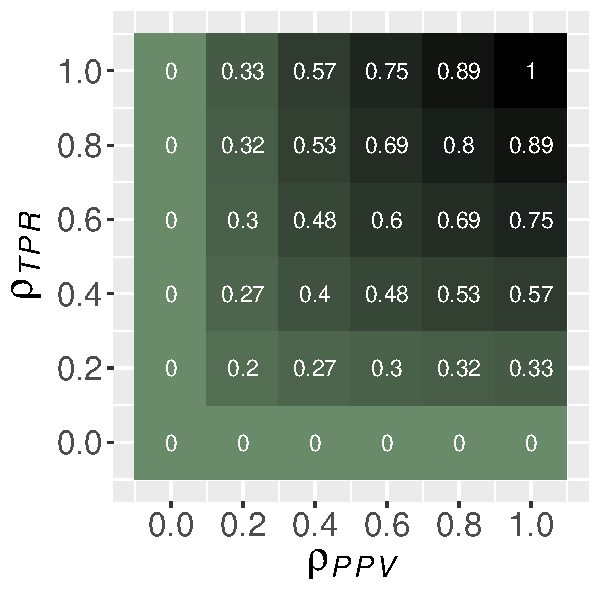
\includegraphics[width=0.8\textwidth]{figure/f1_score_plot.pdf}
	\end{minipage}
	
	\begin{itemize}
		\item A model with $\rho_{TPR} = 0$ (no positive instance predicted as 
		positive) or 
		$\rho_{PPV} = 0$ (no true positives among the predicted) has $\rho_{F_1} = 0$.
		\item Always predicting \enquote{negative}: $\rho_{F_1} = 0$.
		\item [$\leadsto$] No ``$F_1$ score paradox''!
		\item Always predicting \enquote{positive}: $\rho_{F_1} = 2 \cdot \rho_{PPV} / 
		(\rho_{PPV} + 1) = 2 \cdot \np / (\np + n)$,\\ 
		which will be small when the size of the positive class $\np$ is small.
	\end{itemize}
	
\end{vbframe}


\begin{vbframe}{Accuracy Paradox Example: $F_1$ Score}
	%
	\footnotesize
	\begin{itemize}
		%	
		\item Recalling our exemplary setting to illustrate the accuracy paradox:
		%		
		
		\begin{minipage}{0.55\textwidth}    
			%			
			\begin{itemize}
				\scriptsize
				%			
				\item $p(\xv ~| -1) \sim \normal_2\left( 
				\begin{pmatrix}
					0 \\ 0
				\end{pmatrix}  , 
				\begin{pmatrix}
					1  & 0 \\ 0 & 1
				\end{pmatrix}   \right), $
				%		 
				\item  $p(\xv ~| ~ +1) \sim \normal_2\left( 
				\begin{pmatrix}
					0 \\ -2
				\end{pmatrix}  , 
				\begin{pmatrix}
					0.1  & 0 \\ 0 & 0.1
				\end{pmatrix}   \right),  $
				%		
				\item $n_+ = 25,$ $n_- = 1000,$
%				
				\item $f_1(\xv) \equiv -1,$ 
%				
				\item  $f_2(\xv) = 2 \cdot \mathds{1}_{[ \xv \in [-0.66,0.47]\times [-2.74,-1.12] ]} -1.$
				%		
			\end{itemize}
		\end{minipage}
		\begin{minipage}{0.35\textwidth}    
			\begin{center}
				%    	 
				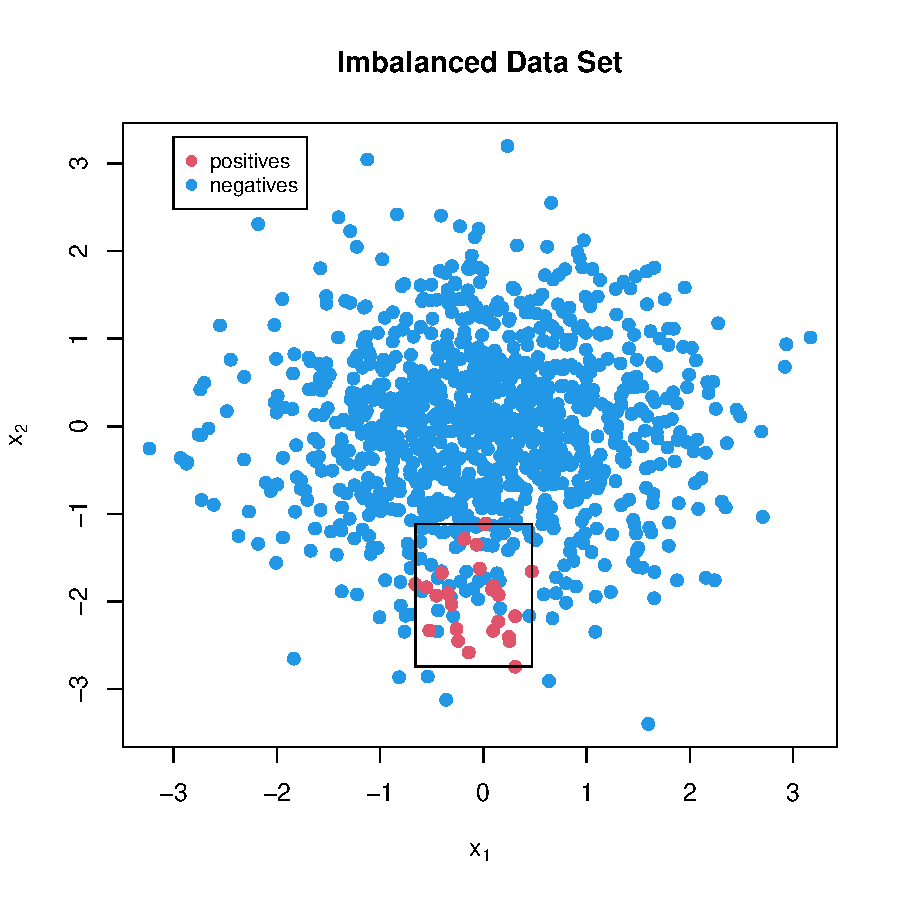
\includegraphics[width=0.8\textwidth]{figure_man/accuracy_paradox}
				%    	
			\end{center}
		\end{minipage}
		%	
		\item $f_1$ has an overall accuracy of $\approx 0.976,$ while $f_2$ has an overall accuracy of $\approx 0.951.$
		%	
		\item The $F_1$ score of $f_1$ is zero, as it has $\rho_{TPR}=0=$ (since $TP=0$), while $f_2$ has  $F_1$ score of $1/2,$ since TP=25, FN = 0 and FP=50, so that $\rho_{PPV}=1/3$ and $\rho_{TPR}=1.$
		%	
		%
	\end{itemize}
	%	
\end{vbframe} 




\begin{vbframe}{G Score}
	\footnotesize
	
	\begin{minipage}[c]{0.5\textwidth}
	\footnotesize
	\begin{itemize}
		\item 	Instead of the harmonic mean in the $F_1$ score one can use also the geometric mean, which results in the G score: 
		%	
		$$\rho_{G} = \sqrt{\rho_{PPV} \cdot \rho_{TPR}}$$
		%	
		\item  Its behavior is similar to the $F_1$ score for different combinations of $\rho_{PPV}$ \& $\rho_{TPR}$, i.e., it tends more towards the lower of the two combined values.
		%	
	\end{itemize}
\end{minipage}%
\begin{minipage}[c]{0.5\textwidth}
	\centering
	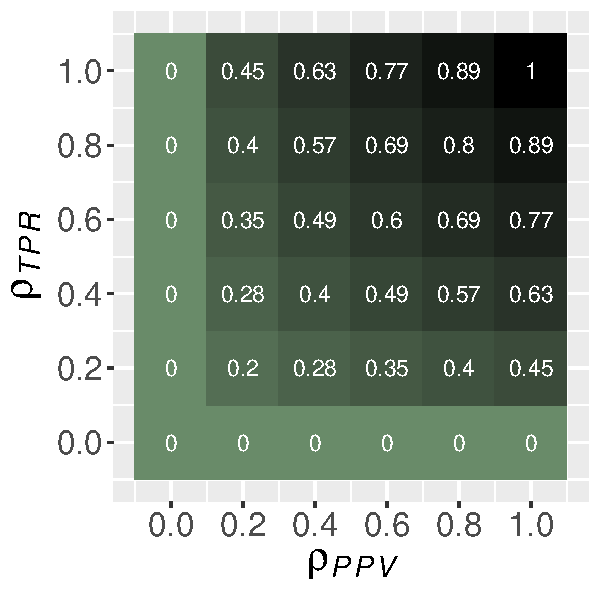
\includegraphics[width=0.8\textwidth]{figure/g_score_plot.pdf}
\end{minipage}
%
\begin{itemize}
	\item %	
	Closely related is the G mean, which uses the geometric mean of TPR and TNR:
	%
	$$\rho_{Gm} = \sqrt{\rho_{TNR} \cdot \rho_{TPR}}.$$
	%	
	It also takes the true negative rate into account, i.e., also true negatives.
%	
	\item For the accuracy paradox example we get a G score of $\approx 0.577$ and a G mean of $\approx 0.975$ for $f_2,$ while $f_1$ achieves G score and G mean of zero, respectively.
%	
	\item Always predicting \enquote{negative}: $\rho_{G} = \rho_{Gm}  = 0 \leadsto$ No ``$G$ score/mean paradox''!
%
\end{itemize}
	
\end{vbframe}



\begin{vbframe}{Balanced Accuracy}
	\footnotesize
	
	\begin{minipage}[c]{0.5\textwidth}
		\footnotesize
		\begin{itemize}
			\item 	Finally, one can also replace the geometric mean in the $G$ mean by the arithmetic mean, which results in the balanced accuracy (BAC): 
			%	
			$$\rho_{BAC} = \frac{\rho_{TNR} + \rho_{TPR}}{2}$$
			%	
			\item  It tends more towards the higher of the two combined values.
			%	
		\end{itemize}
	\end{minipage}%
	\begin{minipage}[c]{0.5\textwidth}
		\centering
		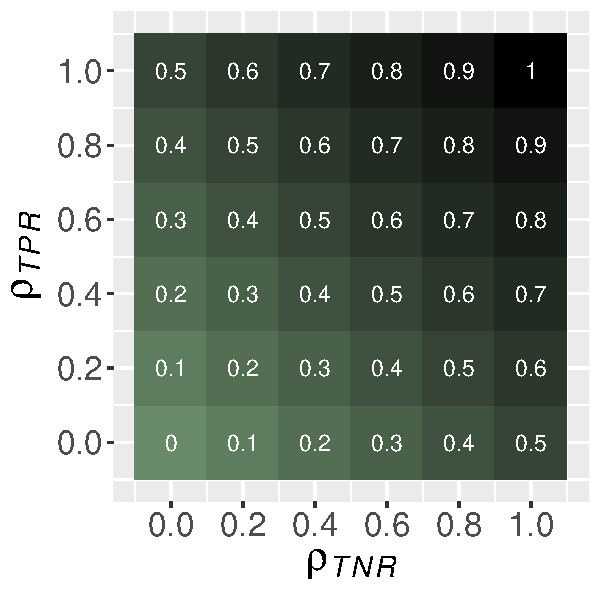
\includegraphics[width=0.7\textwidth]{figure/bac_plot.pdf}
	\end{minipage}
	%
	\begin{itemize}
		\item If a classifier has good predictive accuracy on both classes or the data set is almost balanced, then $\rho_{BAC} $ is essentially the classical accuracy $\rho_{ACC}$.
%		
		\item However, if a classifier always predicts ``negative'' for an imbalanced data set, i.e. $n_+  \ll n_-,$ then $\rho_{BAC} $ is much lower than $\rho_{ACC}$.
		%	
		It also takes the true negative rate into account, i.e., also true negatives.
		%	
		\item For the accuracy paradox example we get a BAC of $0.975$ for $f_2,$ while $f_1$ achieves a BAC of 0.5. As a reminder, $f_1$ has an overall accuracy ($\rho_{ACC}$) of $\approx 0.976,$ while $f_2$ has an overall accuracy of $\approx 0.951.$
		%	
	\end{itemize}
	
\end{vbframe}


\begin{vbframe}{Mattheus Correlation Coefficient}
	%	
	\footnotesize{
	\begin{itemize}
		%
		\item Mattheus Correlation Coefficient (MCC) (aka Phi coefficient) is a measure for the correlation between two binary random variables. In the classification setting the "predicted" classes and the "true" classes are the two discrete random variables:
%		
		$$   \rho_{MCC} = \frac{TP\cdot TN - FP \cdot FN}{\sqrt{(TP+FN)(TP+FP)(TN+FN)(TN+FP)}}$$
		%	
%		
		 \item In contrast to all previous measures the MCC uses all entries of the confusion matrix and its value is in $[-1,1]$ with the following interpretation:
%		 
		\begin{itemize}
			\footnotesize
			%			
			\item $\rho_{MCC} \approx 1$ $\leadsto$ good classification, i.e., strong correlation between correct classifications and true classes.
			%			
			\item $\rho_{MCC} \approx 0$ $\leadsto$ no correlation, i.e., the classification is no better than random guessing.
			%			
			\item $\rho_{MCC} \approx -1$ $\leadsto$ reversed classification, i.e., the classifier is essentially switching the labels.
			%			
		\end{itemize}
		%
	 \item While for the previous measures it is important which class is the positive one (especially in light of imbalanced data), MCC does not depend on which class is the positive one.
%		
	\item For the accuracy paradox example we get an MCC of $\approx 0.563$ for $f_2,$ while $f_1$ achieves an MCC of 0. 
\end{itemize}
		%		
	}
\end{vbframe}


\begin{vbframe}{Performance Measures for Multiclass Classification}
	%	
	\scriptsize{
		%	
		Now consider the multiclass classification setting and the corresponding confusion matrix:
		%	
		\begin{center}
			\tiny
			\begin{tabular}{cc|>{\centering\arraybackslash}p{8em}>{\centering\arraybackslash}p{8em}>{\centering\arraybackslash}p{5em}>{\centering\arraybackslash}p{8em}}
				& & \multicolumn{4}{c}{\bfseries True Class $y$} \\
				& & $1$ & $2$ & $\ldots$ & $g$  \\
				\hline
				\bfseries Classification     & $1$ & $n(1,1)$  &  $n(1,2)$  & $\ldots$ &  $n(1,g)$ \\
				& & (True 1's) & (False 1's for 2's) & $\ldots$ &  (False 1's for $g$'s)  \\
				& $2$ &  $n(2,1)$  &  $n(2,2)$  & $\ldots$ & $n(2,g)$  \\
				$\yh$ & & (False 2's for 1's) & (True 2's) & $\ldots$ &  (False 2's for $g$'s)  \\
				& $\vdots$ & $\vdots$ & $\vdots$ & $\ldots$ & $\vdots$ \\
				& $g$ & $n(g,1)$ & $n(g,2)$  & $\ldots$ &  $n(g,g)$\\
				& & (False $g$'s for 1's) & (False $g$'s for 2's) & $\ldots$ &  (True $g$'s)  \\
			\end{tabular}
		\end{center}
		%	
		Here, $n(i,j)$ is the number of $j$ instances classified as $i$ and $n_i = \sum_{j=1}^g n(j,i)$ the total number of $i$ instances.
%		
		
		We can get multiclass counterparts of the binary evaluation measures by making them class specific: 
		
		\begin{itemize}
			%		
			
			\item True positive rate (\textbf{Recall}): $\rho_{TPR_i} = \frac{n(i,i)}{n_i}$ \quad the fraction of correctly classified instances $i$ among all $i$ instances.
			%		
			\item True negative rate $\rho_{TNR_i} = \frac{\sum_{j\neq i}n(j,j)}{n-n_i}$ \quad the fraction of correctly classified non-$i$ instances among all non-$i$ instances.
%			
			\item Positive predictive value (\textbf{Precision}) $\rho_{PPR_i} = \frac{n(i,i)}{\sum_{j=1}^g n(i,j)},$  the fraction of correctly classified instances $i$ among all $i$ classifications.
%			%		
		\end{itemize}
	}
\end{vbframe}


\begin{vbframe}{Macro $F_1$ Score}
	%	
	\footnotesize{
		%
	\begin{itemize}
%		
		\item In order to obtain a single ``true positive rate'',  ``true negative rate'', or ``positive predictive value'' we can simply average all class-specific rates over all available classes:
		%		
		\begin{itemize}
			\footnotesize
			%			
			\item Macro average true positive rate (macro average precision): $\rho_{mTPR} = \frac{1}{g}\sum_{i=1}^g  \rho_{TPR_i}$
			%			
			\item Macro average true negative rate : $\rho_{mTNR} = \frac{1}{g}\sum_{i=1}^g  \rho_{TNR_i}$
			%			
			\item Macro positive predictive value (macro average recall): $\rho_{mPPR} = \frac{1}{g}\sum_{i=1}^g  \rho_{PPR_i}$
			%			
		\end{itemize}
		%	
		\item With this, one can simply define a macro $F_1$ score by using the harmonic mean of the macro average precision and macro average recall:
		%		
		$$\rho_{mF_1} = 2 \cdot \cfrac{\rho_{mPPV} \cdot \rho_{mTPR}}{\rho_{mPPV} + 
			\rho_{mTPR}}$$
		%	
		\item The problem of this extension for imbalanced data sets is that each class gets an equal weight in the macro average such that the class sizes are not taken into account.
%
	\end{itemize}
	}
\end{vbframe}

\begin{vbframe}{Weighted Macro $F_1$ Score}
	%	
	\footnotesize{
		%
	\begin{itemize}
%		
		\item For imbalanced data sets it is thus better to use a weighted average of the class-specific rates with weights giving more weight to minority classes and few weight to majority classes, i.e., $w_1,\ldots,w_g \in[0,1]$  such that $w_i > w_j$ iff $n_i < n_j$ and $\sum_{i=1}^g w_i = 1.$
%		
		With this, we obtain
		%		
		\begin{itemize}
			\footnotesize
			%			
			\item Macro weighted average true positive rate (macro average precision): $\rho_{wmTPR} = \sum_{i=1}^g  \rho_{TPR_i} w_i$
			%			
			\item Macro weighted average true negative rate : $\rho_{wmTNR} = \sum_{i=1}^g  \rho_{TNR_i} w_i$
			%			
			\item Macro weighted positive predictive value (macro average recall): $\rho_{wmPPR} = \sum_{i=1}^g  \rho_{PPR_i} w_i$
			%			
		\end{itemize}
%	 
		\item Example: $w_i = \frac{n - n_i}{(g-1)n}$ are suitable weights.
		%	
		\item This leads to the weighted macro $F_1$ score:
		%		
		$\rho_{wmF_1} = 2 \cdot \cfrac{\rho_{wmPPV} \cdot \rho_{wmTPR}}{\rho_{wmPPV} + 
			\rho_{wmTPR}}$
		%	
		\item Following this idea, it is straightforward to obtain a weighted macro G score/measure or weighted BAC.
%		
		\item \textbf{Usually} the weighted $F_1$ score is used with weights $w_i = n_i/n,$ i.e., the relative frequency of the $i$-th class in the data set. However, for imbalanced data sets  this is not appropriate as this would give majority classes even more weight.
%
	\end{itemize}
	}
\end{vbframe}


\begin{vbframe}{Other Performance Measures}
	%	
	\footnotesize{
		%
		\begin{itemize}
%			
			\item There are also ``micro'' versions of the $F_1$ score for the multiclass setting, where, for example, the micro weighted average true positive rate (micro average precision) is $\sum_{i=1}^g  \rho_{TPR_i} \frac{1}{n}.$ However, the micro $F_1$ score essentially boils down to the accuracy in this case.
%			
			\item Moreover, the Mattheus Correlation Coefficient (MCC) can be extended to the multiclass setting:
%			
			$$   \rho_{MCC} = \frac{ n  \sum_{i=1}^g n(i,i) -  \sum_{i=1}^g \hat n_i n_i}{\sqrt{ (n^2 - \sum_{i=1}^g \hat n_i^2)(n^2 - \sum_{i=1}^g n_i^2)  }},$$
%			
			where $\hat n_i = \sum_{j=1}^g n(i,j)$ is the total number of instances classified as $i.$
%			
			\item Finally, there are also other performance measures which are based on the idea of treating the "predicted" classes and the "true" classes as two discrete (or categorical) random variables, e.g.\ Cohen's Kappa or Cross Entropy (see Grandini et al.\ (2021)).
			%	
			%		
%			 
%			
		\end{itemize}
	}
\end{vbframe}


\begin{vbframe}{Which Performance Measure to use?}
	%	
	\small{
		%
		\begin{itemize}
			%			
			\item As we have seen, there is a plethora of measures available, which gives rise to the question which of them should be used?	
			%			
			\item  Since all of these measures are focusing on different characteristics of the data, this is a question which in general cannot be answered unambiguously, as this is often depending on the application at hand, which characteristic is more important than another.
			%			
			\item However, it is clear that the usage of accuracy is inappropriate if the data set is imbalanced and another alternative measures should be considered. Usually, the overall picture obtained by the alternative measures will not differ too much.
			%			 
			\item Finally, one needs to be careful by comparing the absolute values of the different measures, as these can be on different ``scales'', e.g.\ MCC and BAC. 
			%			
		\end{itemize}
	}
\end{vbframe}



%
\endlecture
\end{document}
